\documentclass[11pt]{article}
\usepackage[review]{acl}

\usepackage{times}
\usepackage{latexsym}
\usepackage[T1]{fontenc}
\usepackage[utf8]{inputenc}
\usepackage{microtype}
\usepackage{inconsolata}
\usepackage{graphicx}
\usepackage{booktabs}
\usepackage{amsmath}
\usepackage{amsfonts}
\usepackage{multirow}
\usepackage{url}

\title{Adaptive Halting and Evolutionary Latent Control in Recursive Sequence Models:\\Compute Savings, Mechanism Ablations, and Negative Results}

\author{Anonymous Authors}

\begin{document}
\maketitle

\begin{abstract}
We study runtime control of a frozen recursive GRU sequence-to-sequence model in which each output token may undergo up to three latent refinement steps. We first construct a strictly causal, token-level adaptive halting procedure whose compute cost is measured by the exact number of executed base and refinement calls, and show that a simple two-stage confidence threshold retains full exact-match accuracy at 25.7\% of the compute of the deepest fixed depth on three model seeds, passing a held-out confirmation under a preregistered non-inferiority criterion. A pilot comparison with three evolutionary optimizers under identical budgets yields at most 1--2\% additional savings over this threshold. We then ask whether evolutionary computation can instead improve the latent update itself: at fixed depth, evolutionary step-size policies improve inner-subset accuracy by up to +2.1pp over the original update and consistently beat same-budget random search. However, feature ablations show the gains are fully explained by a time-dependent schedule rather than input-dependent state, and one-shot confirmation of joint (step-size + halting) policies fails the non-inferiority criterion on two of three seeds. We report these negative results as the measured boundary of evolutionary latent control on frozen models, together with full preregistration, per-evaluation logs, and reproducibility materials.
\end{abstract}

\section{Introduction}
\label{sec:intro}

Recursive sequence models reapply a refinement operator to a latent state, allowing later iterations to repair earlier mistakes. The benefit, however, is highly uneven: on the COGS semantic parsing task with our frozen GRU model, 87--91\% of examples produce identical output at every refinement depth, while only 5--9\% are repaired by additional refinement. Running the deepest configuration for every token therefore spends most of its compute on tokens that do not need it, and the accuracy--compute trade-off is only meaningful if compute is measured as \emph{actually executed} operations.

This paper studies two runtime control dimensions on such a model. The first is \emph{whether to continue} (adaptive halting): can causally available confidence signals decide, per token, whether further refinement is needed? The second is \emph{how to update} (latent step-size control): can evolutionary computation (EC) discover input-dependent update strengths $\alpha_t$ that improve the latent trajectory itself? We deliberately separate the two: fixed-depth experiments isolate latent-dynamics improvements at constant compute, and joint experiments then test whether such improvements transfer to the accuracy--compute frontier.

Our investigation was governed by preregistered protocols, exact call counting verified by instrumented interception, equal-budget optimizer comparisons with random-search controls, feature ablations for mechanism attribution, and one-shot confirmation of frozen policies. This discipline matters: an earlier internal result reporting 25\% compute cost was invalidated by an audit that revealed look-ahead execution---gates decided after the refinements they were supposed to gate had already been computed. Rebuilding the executor strictly causally, we find the savings are real, but their source is simpler than expected.

We address three research questions:
\begin{itemize}
\item \textbf{RQ1:} Can causal token-level halting maintain task performance while substantially reducing actually-executed refinement compute?
\item \textbf{RQ2:} At fixed depth (constant compute), can EC find latent step-size policies that beat the original update, fixed step sizes, hand schedules, and same-budget random search---and are the gains input-dependent?
\item \textbf{RQ3:} Does jointly optimizing step-size and halting improve the accuracy--compute frontier, and does it survive one-shot confirmation on held-out data?
\end{itemize}

\noindent Our contributions:
\begin{itemize}
\item A strictly causal, token-level adaptive halting procedure with audited compute accounting, evaluated against per-seed frozen depth baselines on three model seeds, with held-out confirmation under a preregistered non-inferiority criterion (\S\ref{sec:exp-halting}).
\item A systematic study of evolutionary latent step-size control on a frozen recursive model, using equal-budget comparisons against random search and feature ablations that attribute the observed gains to a time-dependent schedule rather than input-dependent state (\S\ref{sec:exp-latent}).
\item One-shot confirmation of jointly optimized policies, which fails non-inferiority on two of three seeds; we report this as the current boundary of EC latent control on frozen models, with complete preregistration, per-evaluation logs, and reproducibility materials (\S\ref{sec:exp-joint}, \S\ref{sec:negative}).
\end{itemize}

We deliberately avoid claims that EC ``learned input-dependent dynamics'' or that our confirmation set is untouched data; both are contradicted by our own ablations and data-use audit, and we discuss the implications for evaluation practice in \S\ref{sec:conclusion}.

\section{Related Work}
\label{sec:related}

\paragraph{Adaptive computation and early exit.}
Adaptive Computation Time allocates variable thinking steps to recurrent networks with a learned halting unit \citep{graves2016adaptive}; PonderNet learns a probabilistic halting distribution \citep{banino2021ponder}; the Universal Transformer applies depth-adaptive self-attention \citep{dehghani2019universal}, and depth-adaptive transformers exit per layer or per head \citep{elbayad2020depth}. Our setting differs in two ways: the model is \emph{frozen} (no halting parameters are trained), and all reported compute is the exact count of executed refinement calls, verified by runtime interception rather than derived from exit depths. Anytime and meta-reasoning approaches similarly trade deliberation against cost \citep{zilberstein1996anytime}.

\paragraph{Recursive and iterative refinement models.}
Iterative refinement appears across sequence modeling, from encoder--decoder training \citep{sutskever2014seq2seq,cho2014gru} to repeated latent passes in neural reasoners. The empirical structure we exploit---most examples stable under additional iterations, a small fraction repaired---echoes diminishing per-step returns in iterative inference, but we quantify it as four-way depth transitions (repair/harm/preserve/unresolved) and use it to design the stopping criterion.

\paragraph{Evolutionary computation for neural control.}
EC has been applied to neural weights (neuroevolution) \citep{stanley2019designing} and to controller optimization \citep{eiben2015introduction}. We restrict EC to a five-dimensional step-size policy on a frozen model, which cleanly separates search from representation learning. Our random-search control follows the recommendation that optimizer claims require equal-budget baselines \citep{eiben2015introduction}; our ablations follow mechanism-attribution logic common in analysis-driven research.

\paragraph{Evaluation and confirmation protocols.}
Cluster-robust bootstrap is standard for grouped data \citep{cameron2015practitioner}. We adopt a preregistered non-inferiority criterion (lower 95\% confidence bound of the accuracy difference $\geq -0.5$pp) and one-shot confirmation of frozen policies, inspired by preregistration practice in empirical sciences; the necessity of the confirmation stage is demonstrated empirically by our own negative transfer result.

\section{Method}
\label{sec:method}

\subsection{Recursive GRU Seq2Seq Model}
\label{sec:model}
The model is a GRU encoder--decoder \citep{cho2014gru} in which, at output position $i$, a base step produces a latent state $z_i^{(0)}$ (depth $e_0$). Up to $K{=}3$ refinement steps may follow, each applying a frozen GRU cell $F$ to the current latent:
\begin{equation}
\Delta z_i^{(k)} = F\!\left(\big[\,\mathrm{emb}(y_{i-1});\,c_i;\,e_{\mathrm{soft}}(z_i^{(k)})\,\big],\, z_i^{(k)}\right) - z_i^{(k)},
\qquad
z_i^{(k+1)} = z_i^{(k)} + \Delta z_i^{(k)},
\label{eq:refine}
\end{equation}
where $c_i$ is the encoder context, $e_{\mathrm{soft}}(z)$ the expected embedding under the current output distribution, and $k \in \{0,\dots,K{-}1\}$ indexes refinement steps (depth $e_1$ after one step, $e_3$ after three). Six checkpoints (two model families $\times$ three seeds $s \in \{0,1,2\}$) are frozen; all experiments use family R2.

\paragraph{Empirical depth structure.}
On the gate-training split ($n{=}2{,}419$ per seed), the four-way transition between depths $e_0 \rightarrow e_1$ decomposes into \emph{preserve} (both correct; 87--91\%), \emph{repair} (wrong$\rightarrow$correct; 5--9\%), \emph{unresolved} (both wrong; 3--5\%), and \emph{harm} (correct$\rightarrow$wrong; 0.12--0.25\%). The repair-to-harm ratio of roughly 20--70:1 means recursion is nearly harmless but benefits a minority of examples---exactly the structure under which conservative stopping is safe.

\subsection{Causal Token-Level Adaptive Halting}
\label{sec:halting}
At each token, after the base step (and again after the first refinement), a gate decides whether to stop. Crucially, the decision at each gate may only use signals computed \emph{before} the refinements it gates; the executor never computes a step whose cost is not incurred. Gate~0 (after $e_0$) uses
\begin{equation}
\mathbf{x}^{(0)}_i = \big[\,\mathrm{top}_1,\ \mathrm{margin},\ H,\ \overline{\mathrm{top}}_1,\ p_{75}(H_{\mathrm{hist}}),\ i,\ \mathrm{Var}(\mathrm{top}_1),\ \mathbb{1}[\mathrm{EOS}]\,\big] \in \mathbb{R}^8,
\label{eq:gate0}
\end{equation}
where $H$ is the entropy of the current predictive distribution and the remaining entries summarize the decoded prefix; refinement proceeds iff $\sigma(\mathbf{w}_0^\top \mathbf{x}^{(0)}_i + b_0) \geq \tau_0$. Gate~1 (after $e_1$) uses an analogous 12-dimensional vector that additionally contains the same-state deltas $\Delta\mathrm{top}_1$, $\Delta H$, $\Delta\mathrm{margin}$ and $\lVert z^{(1)}-z^{(0)}\rVert$, and gates the remaining two refinements. The threshold policy in our headline results is the special case ``stop iff $\mathrm{top}_1 \geq \tau$'' with $(\tau_0,\tau_1)=(0.85,0.90)$, preregistered before any evaluation.

\subsection{Actual Computation Accounting}
\label{sec:ncell}
The compute metric is
\begin{equation}
N_{\mathrm{cell}} = \#\{\text{base steps}\} + \#\{\text{refinement calls}\},
\label{eq:ncell}
\end{equation}
summed over a corpus and reported relative to the frozen per-seed best fixed depth (\S\ref{sec:setup}). Correctness is enforced by unit tests (forced stop/continue at each gate yields exactly 0/1/3 refinements per token) and by runtime interception that wraps the refinement module and asserts the counter equals the true call count; forced-depth decoding reproduces frozen training-time trajectories exactly (60/60 samples per depth).

\subsection{Evolutionary Latent Step-Size Control}
\label{sec:alpha}
Separately from halting, we ask whether the update magnitude itself should be input-dependent. We replace \eqref{eq:refine} with
\begin{equation}
z_i^{(k+1)} = z_i^{(k)} + \alpha_i^{(k)}\,\Delta z_i^{(k)}, \qquad
\alpha_i^{(k)} = \sigma\!\big(w_0 + w_1 \tilde H + w_2 \tilde D + w_3 \tilde A + w_4\, k/K\big),
\label{eq:alpha}
\end{equation}
where $\tilde\cdot$ denotes standardization by statistics frozen from $\alpha{=}1$ rollouts on the inner training subset, $H$ the current predictive entropy, $D = \lVert\Delta z\rVert_2/\sqrt{d}$ the previous displacement, and $A$ the cosine between consecutive updates. Setting $\alpha \equiv 1$ recovers the original trajectories exactly (verified token-by-token, 128/128 per seed). All features are causally available at decision time; no gold labels, oracle outcomes, or future-depth signals are used.

\subsection{Joint Control}
A joint policy parameterizes both halting gates (24 dimensions, \S\ref{sec:halting}) and the step-size policy (5 dimensions, \eqref{eq:alpha}), yielding a 29-dimensional genotype decoded by a single procedure in which gate decisions precede the refinements they gate and step sizes modulate each executed refinement.

\subsection{Statistical Criteria}
\label{sec:stats}
All intervals are group-cluster paired bootstrap percentiles \citep{cameron2015practitioner} over structural groups of the task (1{,}000 resamples for development comparisons; 20{,}000 for confirmation, fixed seeds). A policy is \emph{non-inferior} to a baseline iff the lower 95\% confidence bound of the exact-match (EM) difference is $\geq -0.5$pp. Search budgets are exactly 336 candidate evaluations per optimizer (including the initial population), with warm starts from the preregistered threshold policy and per-evaluation best-so-far logs.

\section{Experiments}
\label{sec:experiments}

\subsection{Setup}
\label{sec:setup}
We use the COGS semantic parsing benchmark \citep{kim2020cogs} with a frozen gate split of the training distribution (2{,}419 examples per seed): inner folds (group-clustered, 4/5 of groups) supply search fitness on group-balanced subsets (192--256 examples); a held-out fold (fold-4, 645 examples per seed, group-disjoint from the search folds) is used only for one-shot confirmation of frozen policies. Per-seed frozen best fixed depths are $e_3, e_3, e_1$ for seeds 0--2; all EM differences and compute ratios are relative to each seed's own baseline. The sealed COGS test and generalization sets were never read in any experiment reported here. Optimizers (GA, DE, sep-CMA-ES, random search) share the budget of \S\ref{sec:stats}; the optimizer seed is fixed at 0, so optimizer comparisons are exploratory.

\subsection{Causal Execution and Implementation Validation}
A preregistered engineering audit confirmed: (i) forced-depth decoding matches frozen trajectories exactly (60/60 samples per depth, per seed); (ii) the compute counter equals the true base+refinement call count under runtime interception; (iii) a forced stop at gate 0 executes exactly zero refinement calls; (iv) encoder caching used for throughput leaves all decoded tokens, gate actions, and costs bit-identical. Throughput after caching is 24--42 examples/s on CPU.

\subsection{Adaptive Halting Results (RQ1)}
\label{sec:exp-halting}

\begin{table}[t]
\centering
\small
\begin{tabular}{llccc}
\toprule
Seed / baseline & Policy & $\Delta$EM (pp) & $N_{\mathrm{cell}}$ ratio & Non-inf. \\
\midrule
\multirow{4}{*}{$s_0$ / $e_3$} & threshold & $+0.00$ & 0.2575 & \checkmark \\
 & GA & $-0.31$ & 0.2563 & \checkmark \\
 & DE & $-0.16$ & 0.2563 & \checkmark \\
 & sep-CMA-ES & $-0.31$ & 0.2568 & \checkmark \\
\midrule
\multirow{4}{*}{$s_1$ / $e_3$} & threshold & $+0.00$ & 0.2570 & \checkmark \\
 & GA & $-0.47$ & 0.2537 & \checkmark \\
 & DE & $-0.47$ & 0.2530 & \checkmark \\
 & sep-CMA-ES & $-0.93$ & 0.2553 & $\times$ \\
\midrule
\multirow{4}{*}{$s_2$ / $e_1$} & threshold & $+1.86$ & 0.5212 & \checkmark \\
 & GA & $+2.02$ & 0.5103 & \checkmark \\
 & DE & $-0.31$ & 0.5047 & \checkmark \\
 & sep-CMA-ES & $+2.02$ & 0.5100 & \checkmark \\
\bottomrule
\end{tabular}
\caption{Adaptive halting on the held-out fold ($n{=}645$ per seed), relative to each seed's frozen best fixed depth. EM differences in percentage points; non-inferiority per \S\ref{sec:stats} (full CIs in the appendix). The preregistered threshold policy retains full baseline accuracy at 25.7--25.8\% of $e_3$ compute (seeds 0--1) and exceeds the $e_1$ baseline by 1.86pp at 52.1\% of its compute (seed 2).}
\label{tab:halting}
\end{table}

Table~\ref{tab:halting} shows the RQ1 results. The two-stage confidence threshold is non-inferior on all three seeds while executing 74--75\% fewer refinement computations than the deepest baseline (seeds 0--1) and 48\% fewer than the (already shallow) $e_1$ baseline while \emph{gaining} 1.86pp EM (seed 2). The mechanism is consistent with \S\ref{sec:model}: high-confidence tokens are stable across depths, so stopping on confidence is safe, and low-confidence tokens that continue inherit the deep trajectory's predictions. Equal-budget evolutionary optimizers improve the compute ratio by at most 1--2\% relative over the threshold while remaining non-inferior (except sep-CMA-ES on $s_1$, which exceeds the margin with an all-negative confidence interval); GA and sep-CMA-ES converge to identical behavior on $s_2$. On this model the halting problem is essentially solved by the threshold, and we did not expand the optimizer comparison further.

\subsection{Fixed-Depth Evolutionary Latent Control (RQ2)}
\label{sec:exp-latent}

\begin{table}[t]
\centering
\small
\begin{tabular}{lcccc|ccc}
\toprule
& \multicolumn{4}{c|}{Search (inner EM gain, pp)} & \multicolumn{3}{c}{Ablation (GA, $s_0$)} \\
Seed & RS & GA & DE & sep-CMA & A: $k/K$ & B: $H$ & C: $D,A$ \\
\midrule
$s_0$ & $+0.00$ & $+0.52$ & $+0.52$ & $+0.00$ & $+0.52$ & $+0.52$ & $+0.52$ \\
$s_1$ & $+1.04$ & $+1.56$ & $+1.04$ & $+2.08$ & --- & --- & --- \\
$s_2$ & $+0.52$ & $+0.52$ & $+1.04$ & $+0.00$ & --- & --- & --- \\
\bottomrule
\end{tabular}
\caption{Fixed-depth (constant $N_{\mathrm{cell}}$) improvements over the original $\alpha{=}1$ update on the inner subset ($n{=}192$). All searches use exactly 336 evaluations. Hand schedules (linear decay $1.0\!\rightarrow\!0.5$) and fixed $\alpha \in \{0.75, 0.5, 0.25\}$ never exceed the $\alpha{=}1$ baseline. Ablations on $s_0$ restrict the policy input to a single feature group.}
\label{tab:latent}
\end{table}

At fixed depth the compute is constant, so any EM change is a pure latent-dynamics effect. Table~\ref{tab:latent} shows that EC policies beat the original update on all seeds (up to $+2.08$pp) and beat same-budget random search on all seeds; hand-designed decaying schedules and all fixed step sizes fail. However, the ablations are decisive on mechanism: on $s_0$, restricting the policy to \emph{only} the normalized step index $k/K$, \emph{only} the entropy $H$, or \emph{only} the latent-dynamics features $(D,A)$ each reproduces the full-feature gain exactly ($+0.52$pp). The improvement is a learned one-dimensional mapping---most plausibly a monotone time schedule---and does not require the joint input state. RQ2 is therefore answered with a qualified yes on effectiveness and a clear no on input-dependence.

\subsection{Joint Control and One-Shot Confirmation (RQ3)}
\label{sec:exp-joint}

\begin{table}[t]
\centering
\small
\begin{tabular}{lcc|ccc}
\toprule
& \multicolumn{2}{c|}{Threshold halting (J1)} & \multicolumn{3}{c}{Joint EC policy (J4)} \\
Seed & $\Delta$EM (pp) & ratio & $\Delta$EM (pp) & ratio & Non-inf. \\
\midrule
$s_0$ & $+0.00$ [0, 0] & 0.2575 & $+0.00$ [0, 0] & 0.2564 & \checkmark \\
$s_1$ & $+0.00$ [0, 0] & 0.2570 & $-0.31$ [$-2.3$, $-0.1$] & 0.2539 & $\times$ \\
$s_2$ & $+1.86$ [$-0.5$, $+6.8$] & 0.5212 & $-0.16$ [LCB $< -0.5$] & 0.5061 & $\times$ \\
\bottomrule
\end{tabular}
\caption{One-shot confirmation on the held-out fold ($n{=}645$ per seed) of policies frozen after inner search; brackets are 95\% group-cluster bootstrap CIs of $\Delta$EM (pp) vs.\ the frozen-depth baseline (20{,}000 resamples). J1 passes non-inferiority on all seeds; the best joint EC policy (selected by inner fitness) fails on $s_1$ and $s_2$, losing on $s_2$ the entire EM gain of the threshold policy (paired $\Delta$EM $-2.02$pp vs.\ J1).}
\label{tab:confirm}
\end{table}

Joint search (29 dimensions) improves the inner compute ratio over the threshold by only 0.8--5.7\%, and the crucial question is transfer. Table~\ref{tab:confirm} reports the preregistered one-shot confirmation: the threshold policy passes non-inferiority on all three seeds, whereas the jointly optimized policies---despite favorable inner results (e.g., $+0.52$pp at equal cost on $s_1$)---fail on $s_1$ and $s_2$, and on $s_2$ lose the entire $+1.86$pp held-out gain of the plain threshold. The inner-subset gains of low-dimensional EC controllers do not transfer; RQ3 is answered negatively.

\subsection{Negative Results and Deviations}
\label{sec:negative}
We report the following as first-class findings. (i) The original 25\%-compute claim in our internal history used a look-ahead executor and was invalidated; after rebuilding causally, the number happens to be similar but the evidence is entirely different. (ii) EC latent control does not survive confirmation on frozen models, and its inner gains are schedule-like rather than input-dependent. (iii) Data-use audit: the confirmation fold was previously used in an earlier internal development report of a different experiment line; it was never used for any policy selection, threshold, or hyperparameter in this paper, but ``fully untouched'' claims would be inaccurate. Additional deviations (a warm start outside preregistered bounds, an early-terminated CMA run later completed at full budget with unchanged results, and 51 overlapping examples between an earlier diagnostic and the confirmation fold) are enumerated in the appendix with their resolutions.

\section{Conclusion}
\label{sec:conclusion}
On a frozen recursive GRU model, the reliable way to exploit uneven refinement benefit is a simple, causal, audited confidence threshold: it retains full accuracy at roughly a quarter of the deepest compute on all three seeds and passes one-shot non-inferiority confirmation. Evolutionary search adds at most 1--2\% compute savings to halting, and although it genuinely improves fixed-depth latent updates (beating equal-budget random search), ablations attribute this to a learned time schedule rather than input-dependent dynamics, and jointly optimized policies fail confirmation. Our results suggest that on frozen models the controller-complexity budget is better spent on accounting and confirmation than on richer controllers; making latent refinement control transferable likely requires changing the refinement operator or its training, not post-hoc search. Methodologically, preregistration, exact call counting, equal-budget controls, mechanism ablations, and one-shot confirmation each caught an error that would otherwise have inflated our conclusions; we recommend them as minimum practice for adaptive-computation research.

\section*{Limitations}
Our confirmation fold was used in a prior internal development report (never for policy selection), so confirmation strength is limited; the sealed COGS test/generalization sets remain the only untouched data and were not used. Results are from one dataset, one small GRU architecture, depth $\leq 3$, and single optimizer seeds; optimizer comparisons are exploratory. Ablations were run on one model seed as preregistered. Wall-clock latency does not shrink proportionally with call counts because gating overhead remains; we report call counts as the primary metric. Group definitions used for clustering statistics were built from the full training split's logical forms, though they never enter any policy as input.

\bibliography{references}

\appendix

\section{Reproducibility Materials}
All experiments are preregistered in the repository before execution; each search logs all 336 evaluations with best-so-far curves and genotypes; a 76-check automated consistency audit cross-verifies every number in this paper against raw JSON results; asset SHA-256 hashes, exact commands, environment versions, and the full deviation register are included in the released materials. Checkpoint hashes and the frozen split definition allow exact reproduction of every table and figure. Figures~\ref{fig:pareto}--\ref{fig:traj} visualize the main trade-offs.

\begin{figure}[t]
\centering
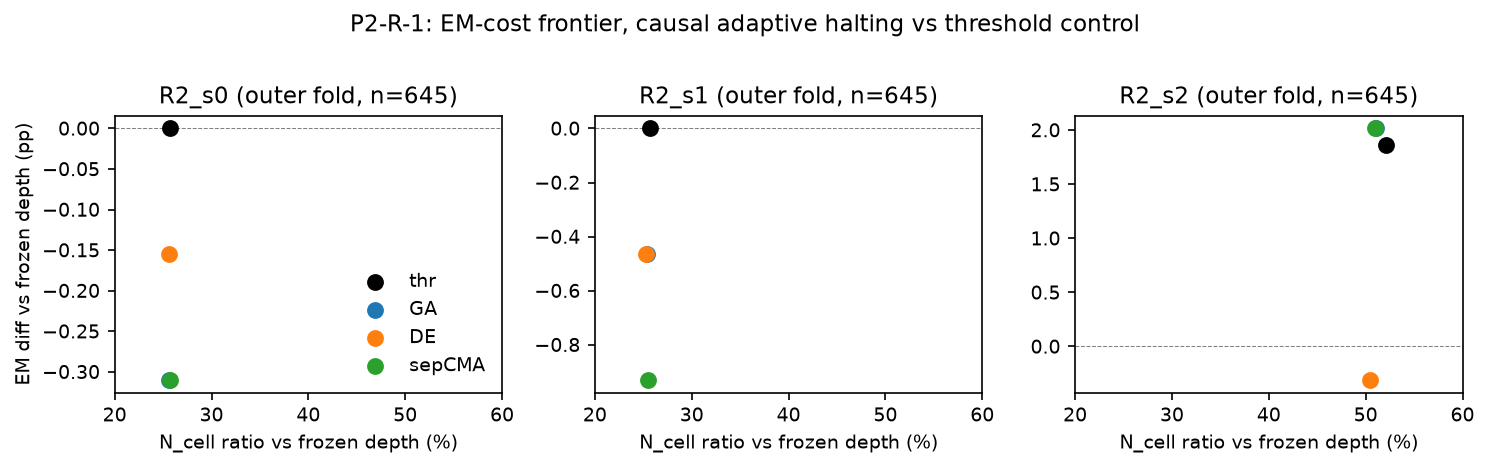
\includegraphics[width=\linewidth]{figures/fig1_p2r1_pareto.png}
\caption{EM--compute frontier on the held-out fold (per seed): threshold vs.\ evolutionary policies.}
\label{fig:pareto}
\end{figure}

\begin{figure}[t]
\centering
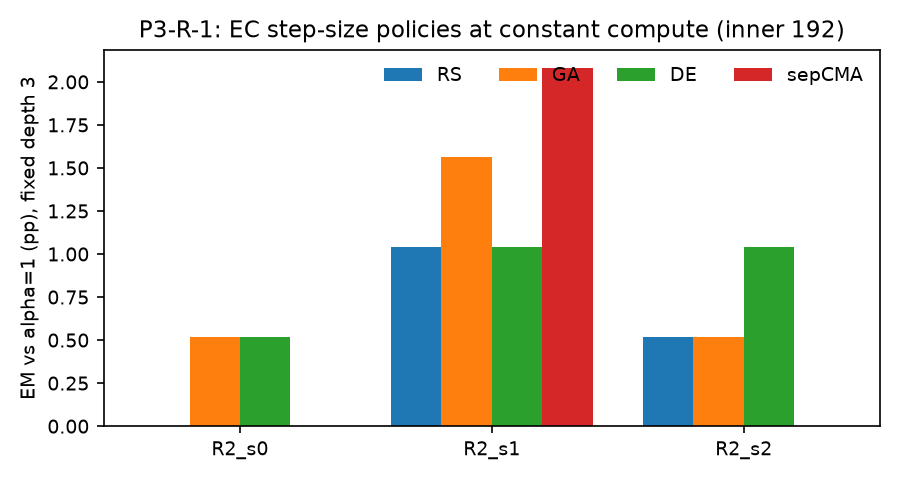
\includegraphics[width=0.8\linewidth]{figures/fig2_p3r1_fixed_depth.png}
\caption{Fixed-depth inner EM gains of EC step-size policies vs.\ $\alpha{=}1$ (constant compute).}
\label{fig:latent}
\end{figure}

\begin{figure}[t]
\centering
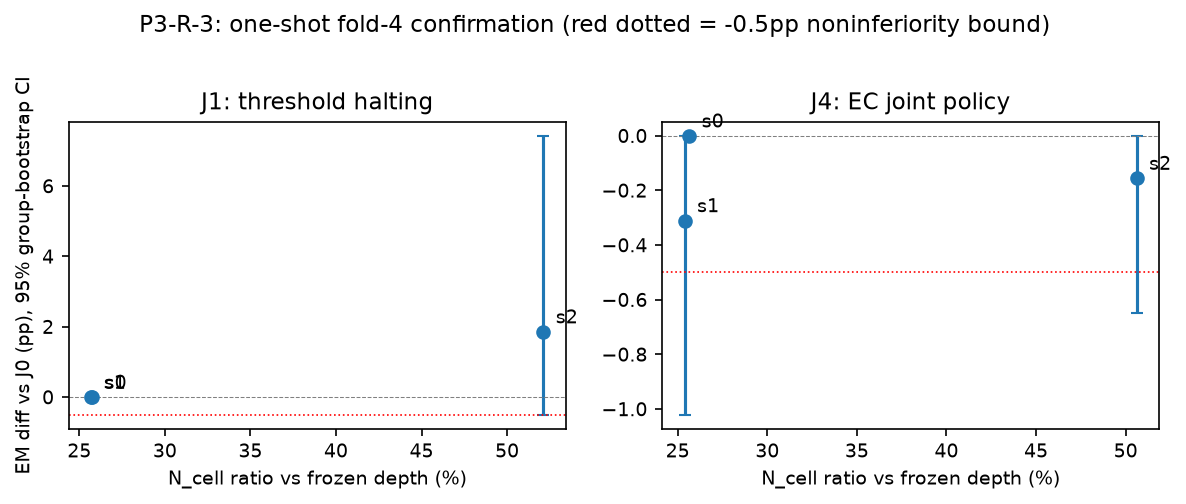
\includegraphics[width=0.9\linewidth]{figures/fig3_p3r3_confirm.png}
\caption{One-shot confirmation with 95\% group-cluster bootstrap CIs; the dotted line marks the $-0.5$pp non-inferiority bound.}
\label{fig:confirm}
\end{figure}

\begin{figure}[t]
\centering
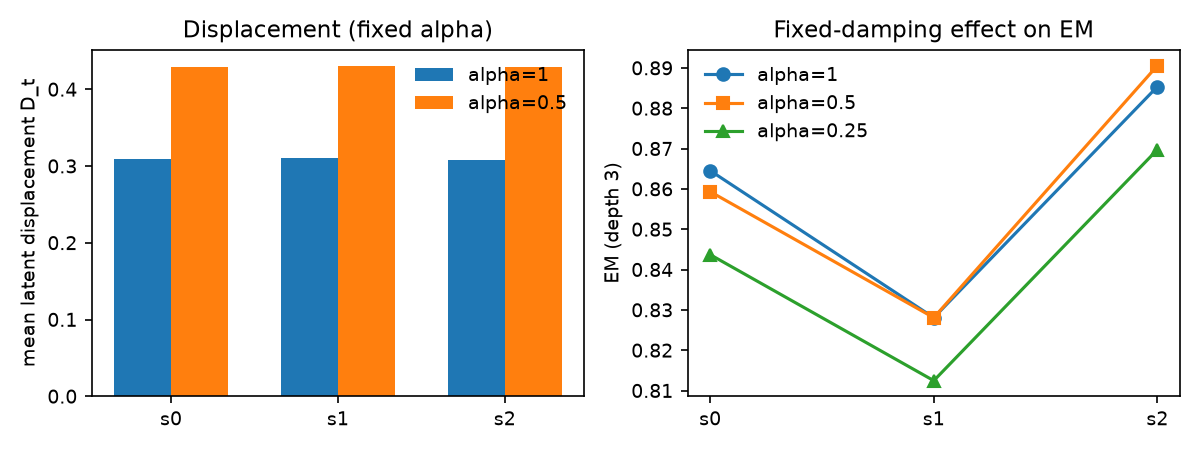
\includegraphics[width=0.9\linewidth]{figures/fig4_p3r0_trajectory.png}
\caption{Latent trajectory statistics under fixed damping.}
\label{fig:traj}
\end{figure}

\section{Full Confidence Intervals}
Per-seed 95\% group-cluster bootstrap CIs for all development comparisons and confirmation results, including compute-ratio intervals and per-sample logs, are provided in the released results archive (JSON/JSONL) and summarized in the repository research report.

\end{document}
